\documentclass[a4paper, 12pt]{article}

\usepackage{hyperref}
\usepackage{fullpage}
\usepackage[top=0.5in, bottom=1.5in, left=0.5in, right=0.5in, footskip=4em]{geometry}
\usepackage{amsmath}
\usepackage{fancyhdr}
\usepackage[usenames,dvipsnames]{xcolor}
\usepackage{pgfornament}

\usepackage[shortlabels]{enumitem}
\usepackage{xspace}
\usepackage{lastpage}
\usepackage{multicol}
\usepackage{blindtext}
\usepackage{titling}
\usepackage{standalone}
\usepackage{amsfonts}
\usepackage[framemethod=TikZ]{mdframed}
\usetikzlibrary{calc}
\usepackage{lineno}
\usepackage{amsthm}
\usepackage{amssymb}
\usepackage{mathtools}
\usepackage{datetime}
\usepackage[most]{tcolorbox}
\usepackage{cancel}
\usetikzlibrary{tikzmark, trees, backgrounds}
\usepackage{pgfplots}
\linenumbers
\usepackage{tikz-qtree}

%BEGIN_FOLD Commands
\usepackage{amssymb}% http://ctan.org/pkg/amssymb
\usepackage{pifont}% http://ctan.org/pkg/pifont
\newcommand{\cmark}{\ding{51}}%
\newcommand{\xmark}{\ding{55}}%
\newcommand{\half}{\ensuremath{\frac{1}{2}}}
\newcommand{\epv}[1]{\ensuremath{\left< #1 \right>}\xspace}
\newcommand{\variance}{\ensuremath{\text{Var}}}
\newcommand{\eout}{\ensuremath{E_\text{out}}\xspace}
\newcommand{\ein}{\ensuremath{E_\text{in}}\xspace}
\newcommand{\cx}{\ensuremath{\mathcal{X}}\xspace}
\newcommand{\cz}{\ensuremath{\mathcal{Z}}\xspace}
\newcommand{\real}{\mathbb{R}}
\DeclareSymbolFont{extraup}{U}{zavm}{m}{n}
\DeclareMathSymbol{\varheart}{\mathalpha}{extraup}{86}
\DeclareMathSymbol{\vardiamond}{\mathalpha}{extraup}{87}
\renewcommand{\heartsuit}{\textcolor{red}{\varheart}}
\renewcommand{\diamondsuit}{\textcolor{red}{\vardiamond}}
\newcommand{\definition}{\vspace{1em}\noindent\textbf{Def:} }
\newcommand{\theorem}{\vspace{1em}\noindent\textbf{Theorem:} }
\newcommand{\example}{\vspace{1em}\noindent\textbf{Example:} }
\newcommand{\solution}{\newline\noindent\textbf{Solution:} }
\newcommand{\predicate}{\vspace{0.25em}\noindent\textbf{Inductive Predicate:} }
\newcommand{\inductivestep}{\vspace{0.25em}\noindent\textbf{Inductive Step:} }
\renewcommand{\proof}{\vspace{0.5em}\noindent\textbf{Proof:} }
\newcommand{\lemma}{\vspace{1em}\noindent\textbf{Lemma:} }
\newcommand{\hint}{\textbf{Hint:} }
\newcommand{\basecase}{\vspace{0.25em}\noindent\textbf{Base Case:} }
\newcommand{\inductivehypothesis}{\vspace{0.25em}\noindent\textbf{Inductive Hypothesis:} }
\newcommand{\collorary}{\vspace{1em}\noindent\textbf{Collorary:} }
\newcommand{\qedd}{\qed\newline}
\newcommand{\kwd}[1]{\textcolor{blue}{\textbf{\underline{#1}}}}
\newcommand\ColorBox[2][]{%
	\stepcounter{mybox}%
	\node[draw=red!70!black,fill=red!20,align=left,#1] (box\themybox) {#2};
}
\newcommand{\expl}[2]{%
	\underset{\substack{\uparrow\\\mathrlap{\text{\hspace{-1em}#2}}}}{#1}}
\newcommand{\uexpl}[2]{%
	\overset{\substack{\mathrlap{\text{\hspace{-1em}#2}}\\\downarrow}}{#1}}
\newcommand{\st}{\text{ such that }}
\newcommand{\R}{\textcolor{red}{R}}
\newcommand{\sumn}{\sum^n_{i=0}}
\newcommand{\sumxn}{\sum^n_{x=0}}
\newcommand{\red}[1]{\textcolor{red}{#1}}
\newcommand{\blue}[1]{\textcolor{blue}{#1}}
%\newcommand{\qed}{\ensuremath{\blacksquare}}
%END_FOLD
\newcommand{\sidenote}[1]{\textcolor{gray}{#1}}
\let\Pr\relax
\DeclareMathOperator{\Pr}{Pr}
%BEGIN_FOLD miscellaneious default
\makeatletter
% Make a copy of macros responsible for entering display math mode
\let\start@align@nopar\start@align
\let\start@gather@nopar\start@gather
\let\start@multline@nopar\start@multline
% Add the "empty line" command to the macros
\long\def\start@align{\par\start@align@nopar}
\long\def\start@gather{\par\start@gather@nopar}
\long\def\start@multline{\par\start@multline@nopar}
\makeatother
\setlength{\columnsep}{1cm}
%opening
\setlength{\abovedisplayskip}{-\baselineskip}%
\setlength{\abovedisplayshortskip}{\abovedisplayskip}%

\pagestyle{fancy}
\renewcommand{\headrulewidth}{0pt}
\lfoot{\small{\course}: Week \weekno}
\rfoot{\small{\thetitle}}
\rhead{}
\cfoot{\pgfornament[height=1em, ydelta=-0.4em]{17} \thepage of \pageref{LastPage}  \pgfornament[height=1em, ydelta=-0.4em]{18}}

\DeclareMathOperator{\sign}{sign}
\newcommand{\vect}[1]{\ensuremath{\mathbf{#1}}\xspace}

\tikzstyle{every picture}+=[remember picture]
\newcommand{\bwgrid}[1]{
	\def \aaa #1
	
	\foreach \y in {0,1,2} {
		\foreach \x in {0,1,2} {
			\pgfmathsetmacro{\clr}{\aaa[\x][\y]}
			%\message{aaa \clr}
			\definecolor{MyColor}{rgb}{\clr,\clr,\clr}
			\path[fill=MyColor] (\x,\y) rectangle ++(1,1); 
		}
	}
	\draw[step=1cm,very thin] (0,0) grid (3,3);	
}

\setenumerate{label=\alph*.)}
\definecolor{db}{RGB}{100,65,23}

%END_FOLD

\newcommand{\course}{Discrete Math}
\title{Probablility}
\newcommand{\weekno}{8}

\begin{document}
\begin{center}
	\textcolor{orange}{\textsc{\course}}\\
	\huge\textbf{\textsc{\thetitle}}\\
	\small\textcolor{gray}{Last updated:\, \today \, \currenttime}\\
	\pgfornament[width=0.7\textwidth, color=white!30!black]{88}
\end{center}


\begin{multicols}{2}
Let us get the intuitive idea behind the probability before we get to the formal definition. 

\section*{Monty Hall Problem}

The first example is based on an American game show in 1980's called . It is called Monty Hall problem named after the host of the game show Monty Hall.

The game show goes like the following: you are given three doors to choose. There is a car behind one of the door and behind the other two door has goats behind it.
\begin{itemize}
	\item First, the player pick a door.
	\item Since there are two empty doors, at least one empty door is not picked. The host will then open one of the empty door that is not picked by the player.
	\item The host then ask the player whether to switch the door he pick to the other non open door or not.
\end{itemize}
The question is should the player switched or not.

This problem can be explaind easily by just drawing a tree.
\end{multicols}

\includestandalone[]{montyhall}


From the picture, to calculate the probably that you switch and win, all we need to do is add up all the probability of the sample that you win.
\begin{align*}
	\Pr(\text{switch and win}) = &\Pr([A,B,C]) + \Pr([A,C,B]) + \Pr([B,A,C]) +\\ &\Pr([B,C,A]) + \Pr([C,A,B]) + \Pr([C,B,A])\\
	=&6 \times \frac{1}{9} = \frac{2}{3}
\end{align*}

\begin{multicols}{2}

Thus, the probability of switch and win is $\displaystyle \frac{2}{3}$ and the probability of not switch and win is $\displaystyle \frac{1}{3}$. So, you should switch.

One way to understand this seemingly counterintuitive result is that if we switch the door we are essentially picking two doors. So, the chance should really be twice as much.

The confusion usually comes from the fact of what is being define of equal probability. Naively one would think that each outcome have the same probability associated with it. But, in fact, each outcome do not have the associated probability as you can see from the tree we drew.
\section*{Strange Dice}

Let us consider another example. The three dices have the following faces
\begin{align*}
	\text{Dice A} &= {2,6,7}\\
	\text{Dice B} &= {1,5,9}\\
	\text{Dice C} &= {3,4,8}
\end{align*}

The rule of the game is simple. There are two players each one pick a dice who ever roll greater number wins.

By drawing a tree(I would if i have time), one can conclude
\begin{itemize}
	\item $A$ wins $B$ with probability of $5/9$
	\item $B$ wins $C$ with probability of $5/9$
	\item ans surprisingly $C$ wins $A$ with probability of $5/9$
\end{itemize}

This show that probability does not have the associative probability.


\section*{Formal Definition}

\definition A countable(just means the set where you can list the members) \kwd{sample space} $S$ is a non-empty countable set. An elements $\omega \in S$ is called an \kwd{outcome}.

For example, for tossing a coint two times, the same space would be
\[
	S = \{HH, HT, TH, TT\}
\]

\definition A \kwd{probability function} is a function $Pr: S \to \real$ such that
\begin{itemize}
	\item $\Pr[\omega] \ge 0$ $\forall \omega \in S$. Probability associated with an outcome cannot be negative.
	\item $\displaystyle \sum_{\omega \in S} \Pr[\omega] = 1$. The sum of all probability is 1.
\end{itemize} 

The probability for the two coin toss, the probability function would be
\begin{align*}
	\Pr[HH] = \Pr[HT] = \Pr[TH] = \Pr[TT] = 0.25
\end{align*}


\definition A \kwd{probability space} is the sample space together with probability function.

For example, the probability space would be $(S, Pr)$ where
\begin{equation*}
	S = \{HH, HT, TH, TT\}
\end{equation*}
and the probability function
\begin{equation*}
	\Pr[HH] = \Pr[HT] = \Pr[TH] = \Pr[TT] = 0.25
\end{equation*}

\definition An \kwd{event} is a subset of a samplespace.\[
 E \subseteq S
\]
For example, an event where the two coin toss give the same face
\[
	E = \{ HH, TT\}
\]

\definition We can then define the probablity on the event as the sum of all the outcome in the event.
\[
	\Pr[E] = \sum_{\omega \in E} \Pr[\omega]
\]
For example, the probability that the two tosses come up the with the same face is
\[
	\Pr[\{HH, TT\}] = \Pr[HH] + \Pr[TT] = 0.5
\]

These definitions match with what our intuition says about probability. We can retrace what we did in the montehall case and the strange dice case to these definitions.

The sample space may not be a finite set. For example, let us consider a game of two player fair coin toss. The two players alternate the coin toss. Whoever get the first head wins. For instance, if the first player get head the first time he toss. He just win and the game ends.

\begin{tikzpicture}[grow'=right]
	\node{} 
	child{
		node[] {T} 
		child{
			node {T}
			child{
				node {T}
				child{
					edge from parent[dashed]
				}
				child{
					node {H}
				}	
			}
			child{
				node {H}
			}	
		}
		child{
			node {H}
		}		
	}
	child{
		node[] {H}	
	};
\end{tikzpicture}

The sample space for this game would be
\[
S = \{H, TH, TTH, TTTH, TTTTH, \ldots\}
\]. The sample space is infinite. The probability of each one looks like  $\Pr[H] = 1/2$, $\Pr[TH] = 1/4$, $\Pr[TTH] = 1/8$, etc. 

Now we want the calculate the probability that the first player wins. The event that the first player win is \[
E = \{H, TTH, TTTTH, TTTTTTH, \ldots \}
\]

This means the probability of the first player winning is
\begin{align*}
	\Pr[E] &= \Pr[H] + \Pr[TTH] + \Pr[TTTTH] + \ldots\\
	&= \frac{1}{2} + \frac{1}{2^3} + \frac{1}{2^5} + \frac{1}{2^7} + \frac{1}{2^9}+\ldots \\
	&= \frac{1}{2} \left( 1 + \frac{1}{2^2} + \frac{1}{2^4} + \frac{1}{2^6} + \frac{1}{2^8} + \ldots \right)\\
	&= \frac{1}{2} \left( 1 + \frac{1}{4} + \frac{1}{4^2} + \frac{1}{4^3} + \frac{1}{4^4} + \ldots \right)\\
	&= \half \left(\frac{1}{1-\frac{1}{4}}\right)\\
	&= \frac{2}{3}
\end{align*}

\section*{Common sense rule.}

Since the probabilty of an event is just a linear sum of probability of all outcome in the event set. A lot of cardinality rule we learn from counting works here too.

\subsubsection*{Sum Rule}
For example, if $E_1$ and $E_2$ are disjoint ($E_1\cap~E_2=\emptyset$) then
\[
	\Pr\left[E_1 \cup E_2\right] = \Pr[E_1] +  \Pr[E_2]
\]

\begin{center}
	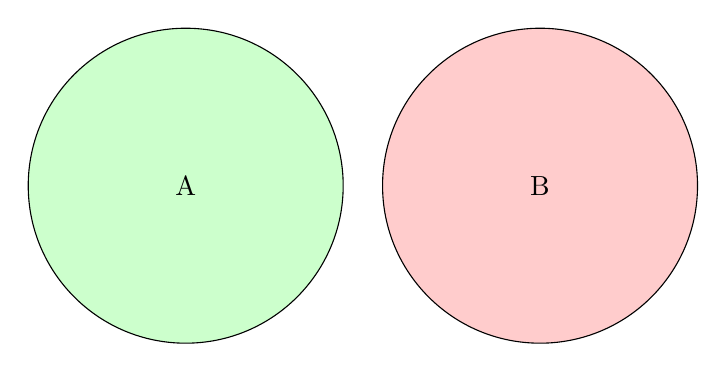
\begin{tikzpicture}
	\draw[fill = green, fill opacity=0.2] (0,0) coordinate (A) circle (2 cm) node[fill opacity=1] {A};
	\draw[fill = red, fill opacity=0.2] (4.5,0) coordinate (B) circle (2 cm) node[fill opacity=1] {B};
\end{tikzpicture}
\end{center}

This is quite intuitive. Suppose I give you 1 yoyo at random. You have certain probability of getting a red yoyo and a certain probability of getting pink yoyo. The probability of getting pink yoyo or red yoyo is then just the sum of the two probability.

\subsubsection*{Complement Rule}
The probability of something not happens is just one minus the probability of that event happens.
\[
	\Pr(\bar{E}) = 1 - Pr(E)
\]

For example, the probability of not raining today is just one minus the probability of raining.

\subsubsection*{Difference Rule}
The probability of B happens but not A is just the probability that B happens minus the probability that both A and B happens.
\[
	\Pr(B-A) = \Pr(B) - \Pr(B \cap A)
\]

\begin{center}	
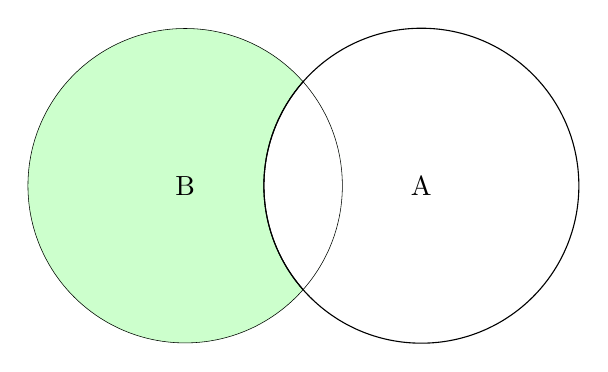
\begin{tikzpicture}
\begin{scope}
\clip (0,0) circle (2 cm);
\draw[fill = green, fill opacity=0.2, even odd rule] (0,0) circle (2 cm) node[fill opacity=1] {B} (3,0) coordinate (B) circle (2 cm);
\end{scope}
\draw[] (B) circle (2 cm) node[fill opacity=1] {A};
\end{tikzpicture}
\end{center}

\subsubsection*{Union Rule}
All the inclusion-exclusion rule works here too. For example,
\[
	\Pr\left[E_1 \cup E_2\right] = \Pr[E_1] +  \Pr[E_2] - \Pr[E_1 \cap E_2]
\]

\section*{Conditional Probability}

Most of the time the probability that you are interested in is the probability of something happens given some information. Consider picking a random person in Thailand. The probability of that person being an MUIC student would be
\[
	\Pr(\text{MUIC Student}) = \frac{\text{\# MUIC Student}}{\text{\# People in Thailand}}
\]

But, now if we ask that person where does he/she lives and the answer is Nakornpathom, then it is clear the the probability that he/she is an MUIC student would be much higher. So, this kind of probability is called conditional probability: the probability of something given some information. Specifically, the probablity of some one being an MUIC student given that he/she lives in Nakornpathom(NKP) is denoted by
\[
	\Pr(\text{MUIC Student} | \text{Live in Nakornpathom})
\]

We can visualize that probability as
\begin{center}
	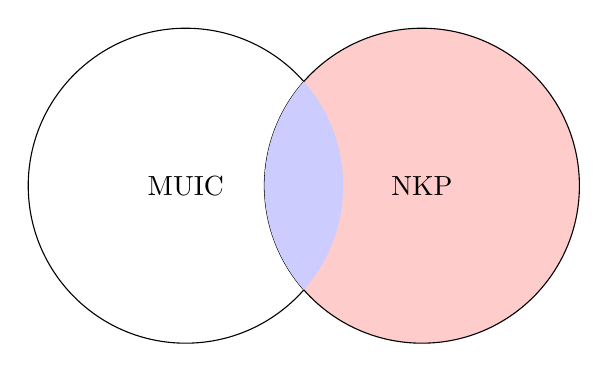
\begin{tikzpicture}
		\draw (0,0) circle (2cm) node {MUIC};
		\draw[fill=red!20!white] (3,0) circle (2cm) node{NKP};
		\begin{scope}
		\clip (0,0) circle (2cm);
		\fill[blue!20!white] (3,0) circle (2cm);
		\end{scope}
	\end{tikzpicture}
\end{center}

This means that the probability we want to calculate is the number of people who lives in the NKP and study at MUIC (blue region) normalized by all the people live in Nakornpathom (blue and red region).
\[
	\Pr(\text{MUIC}|\text{NKP}) = \frac{\text{\# (MUIC $\cap$ NKP)}}{\text{\# NKP}}
\]

With this notion we can define the conditional probability as

\definition The probability of event $A$ given event $B$, $Pr(A|B)$, is given by
\[
	\Pr(A|B) = \frac{\Pr(A \cap B)}{\Pr(B)}
\]
This is quite important law in probability that it is given a name Bayes's rule.

\subsection*{Soccer Match}

Let us look at an example. Suppose you are in a soccer game, you have to win 2 out of 3 games to win. The probability of you winning the first game is $1/2$. But, if you win one game the next game the probability of winning again is $2/3$ due to mysterious morale boost. From this situation you can draw the tree as

\begin{center}
	\includestandalone{soccermatch}
\end{center}

From the picture above, the probability of winning is
\[
	\Pr(\text{Winning}) = \frac{1}{3} + \frac{1}{18} + \frac{1}{9} = \half
\]

But we want to know more. If we happen to win in the first match(WFM), we want to know the probability that we will win the tournament(WT). The probability that we want to calculate is, by Bayes' rule,
\begin{align*}
	\Pr(\text{WT} | \text{WFM}) &= \frac{\Pr(WT \cap WFM)}{\Pr(WFM)} \\
	&= \frac{\frac{1}{3} + \frac{1}{18}}{\frac{1}{2}}\\
	&= \frac{7}{9}
\end{align*}

You can do a similar thing and find that the probability of losing the tournament given that you win the first round is $\displaystyle \frac{2}{9}$

We can ask \emph{a posteriori} question, which is a fancy word meaning reverse in time. For example, we can ask the question that given that we in the tournament, what is the probability that we win the first round. We can also calculate this using Bayes's rule:
\begin{align*}
	P(\text{WFM}|\text{WT}) =& \frac{\Pr(WT \cap WFM)}{\Pr(WT)}\\
	=& \frac{\displaystyle \frac{1}{3} + \frac{1}{18}}{\displaystyle \frac{1}{3} + \frac{1}{18} + \frac{4}{18}}\\
	=& \frac{7}{11}
\end{align*}




\subsection*{Tree Diagram}
The bayes rule is also the reason by the tree diagram we drew works. We try to compute the probability that the all the event in the branch leading to the leaf is. The probability that we write on each edge is just the probability that something happens given all the other things leading to that edge happen. For example, we do this without even thinking about it
\begin{align*}
	\Pr(A \cap B) &= \Pr(B) \cdot \Pr(A|B)\\
	\Pr(A \cap B \cap C) &= \Pr(C) \cdot Pr(B|C) \cdot \Pr(A | B \cap C)
\end{align*}

%Todo: Add picture here in the future.

\subsection*{Medical Trial}

Let us consider a medical test for a disease that have the following sensitivity and specificity.
\begin{itemize}
	\item \kwd{Sensitivity}. If you have the disease, then there is 90\% chance that the test will tell you that you have the disease. This is also called a true positive rate.
	\item \kwd{Specificity}. If you \emph{do not} have the disease then there is a 70\% chance that the test will tell you that you \emph{do not} have a disease. This is also called the true negative rate.
	\item 10\% of the population have the disease.
\end{itemize}

\begin{center}
	\includestandalone{medicaltest}
\end{center}

An important question to ask is that if you get the test and the test says you are positive(PT) what is the probability that you do have the disease(D).
\begin{align*}
	\Pr(D|PT) =& \frac{\Pr(D \cap PT)}{\Pr(PT)}\\
	=& \frac{0.1 \times 0.9 }{0.1\times 0.9 + 0.9 \times 0.3}
	=& 25\%
\end{align*}
So, even though you should be a bit worried more than when you didn't have the test(10\%). You should not be too much worried since the probability of you having the disease given that the test is positive is just $25\%$.

Let us calculate the probability of the test being correct.

I can be correct more often just just keep saying no. But that is not a very useful test. So, the ``correctness" is not the measure of how useful a test is. There is really no right answer for this. It is all depend on what is the cost of the false negative and the cost of false positive. If the disease you are diagnosing is an contagious zombie disease then false negative would cost you a lot: end of humanity while false postive doesn't cost much. Whereas if the disease we are talking about is just a mild disease that we can fix when the true symptom occur  but it costs a lot money to cure, then one false positive would cost a lot, while false negative doesn't really matter we can just wait until the symptom occur and fix it.

\subsection*{Yoyo Box}

Suppose I have 2 boxes of yoyo.
\begin{itemize}
	\item One box has a cola yoyo and a grape yoyo. The other box has 2 cola yoyo.
	\item I then pick a box at random.
	\item Then, we randomly draw a yoyo from the box we chose. 
	\item If the yoyo we drew is a grape yoyo, then we randomly pick a box again.
	\item If the yoyo we drew is a cola, then we play the game by drawing the other yoyo from the box. If it comes out grape you win, and if it comes out cola I win.
\end{itemize}

We can analyze the game again using the tree diagram. What we want to find is the probability that the box we pick is the one with two flavors given that the first yoyo we drew is a cola.

\begin{center}
	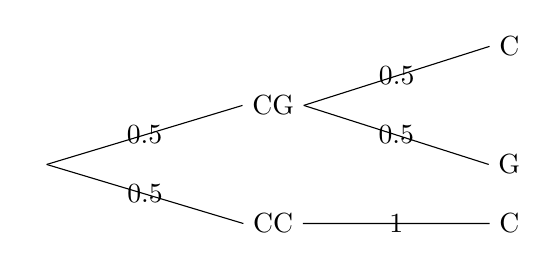
\begin{tikzpicture}[grow'=right, level 1/.style={level distance=3cm}]
	\node{}
	child{
		node{CG}
		child{
			node{C}
			edge from parent node{0.5}
		}
		child{
			node{G}
			edge from parent node{0.5}
		}
		edge from parent node{0.5}
	}
	child{
		node{CC}
		child{
			node{C}
			edge from parent node{1}
		}
		edge from parent node{0.5}
	};
\end{tikzpicture}
\end{center}

Of course, none of the game you play in this class is fair. AJ always cheat. The probability of the box we pick is CG(Cola Grape) given that the yoyo we draw is a Cola is
\begin{align*}
	\Pr(CG|C) =& \frac{\Pr(CG \cap C)}{C}\\
	=& \frac{ \frac{1}{4}}{ \frac{3}{4}}\\
	=& \frac{1}{3}
\end{align*}
This means AJ wins with the probability of $\displaystyle \frac{2}{3}$
This is not a fair game. As an exercise you should think about whether having 2 CG boxes and 1 CC box make the game a fair game.

\subsection*{Conditional Probability Properties}
These can be understand quite easily by just drawing a diagram.
\[
\Pr(A) = \Pr(A|E)\cdot \Pr(E) + \Pr(A|\bar{E})\cdot \Pr(\bar{E}) 
\]
This reads the probabilty of event $A$ is the sum of the probabilty of event $A$ happen given $E$ times probability that $E$ happens and the one where $E$ doesn't happen. This is called the law of total probability.

Also, you can conditioning on the intersection and it works like it should since we just change the normalization.
\[
	\Pr[A \cup B | C] = \Pr[A | C] + \Pr[B|C] - \Pr[A\cap B | C]
\]

However, one need to be careful about conditioning on the union.
\[
	\Pr[C | A \cup B] \ne \Pr[C|A] + \Pr[C|B]
\]
A counterexample can be shown using the figure below
\begin{center}
	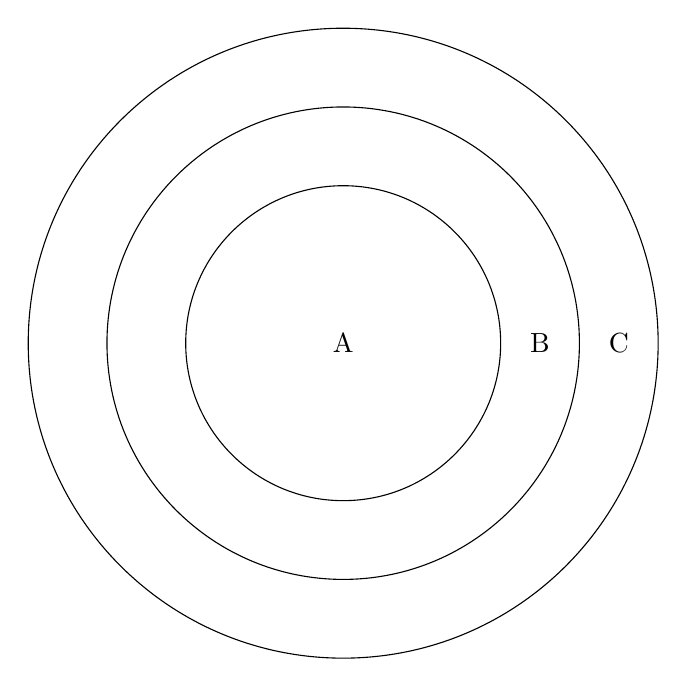
\begin{tikzpicture}
	\draw (0,0) circle (2cm) node {A};
	\draw (0,0) circle (3cm) node [xshift=2.5cm] {B};
	\draw (0,0) circle (4cm) node [xshift=3.5cm] {C};
\end{tikzpicture}
\end{center}
From the picture $\Pr[C|A]=1$ since $C$ is guarantee to happen if $A$ happen. Also, $\Pr[C|B]=1$ for the same reason. So, if we add the two up we will get 2 which is not a probability.



\section*{Simpson Paradox}
Consider the following table for the ontime rate for American Airlines(AA) and American West Airlines(AW). The question is which one should you fly?

\begin{center}
	\begin{tabular}{|c|c|c|c|c|}
	\hline  & AA &  & AW &  \\ 
	\hline LA & 500/560 & 89\% & 700/800 & 87\% \\ 
	\hline PHO & 220/230 & 95\% & 4900/5300 & 92\% \\ 
	\hline SD & 210/230 & 92\% & 400/450 & 89\% \\ 
	\hline SF & 500/600 & 83\% & 320/450 & 71\% \\ 
	\hline Seattle & 1900/2200 & 86\% & 200/260 & 77\% \\ 
	\hline\hline Total & 3300/3820 & 87\% & 6520/7260 & 90\% \\ 
	\hline 
\end{tabular} 
\end{center}

The peculiar thing about this table is that even though AA is better than AW in every single airport the total rate for AA is worse than AW. You can ask the question that given that you will be flying off from LA, what is the airline we should choose? Clearly it is AA. You can ask this question for every single airport, the answer will always be AA.

However, if you do not know where you are flying off, you will be better off with AW.

This results is called Simpson's Paradox. Newspaper do this all the time. But, since you have learned this, I hope whenever you see someone totalling the ratio, you will notice the pitfall.



%There is also another two words that you may encouter in your career.
%\begin{itemize}
%\item The false negative rate which is the rate that you do have the disease but the test tell you that you do not have the disease. This is just $1-90\% = 10\%$
%\item The false positive rate which is the rate that the test tell you that you have the disease but you \emph{do not} have the disease. This is just $1-70\% = 30\%$
%\end{itemize}
%The choice of which two to tell depends on the field but the important thing is you know what it means.

\section*{Independence}

\definition Event $A$ and event $B$ are independent iff
\[
	\Pr(A|B) = \Pr(A) \;\text{  or  }\; \Pr(B)=0
\]
In other word, given the information about $B$ does not tell you anything about $A$.

For example, let us consider tossing two fair coins consecutively. Let us consider two events
\begin{itemize}
	\item Event $A$. The two coins are the same.
	\item Event $B$. The first coin is head.
\end{itemize}
Are $A$ and $B$ independent?

All we need to do is checking whether $\Pr(A|B)$ and $\Pr(A)$ are equal. The probability that the coins are the same($\Pr(A)$) is $1/2$. If the first coin is head then the probability that the two coins are the same is the probability that the second coin is also head so $\Pr(A|B)=1/2$. So, event $A$ and event $B$ are independent.

It should also be noted that using fair coin doesn't imply the fact that the result of the two coins are independent. You can tape the coins together. The two events are still independent.

What if the coin is not fair? This means that the probability of getting head is $p$ and the probability of getting tail is $1-p$. Would the two event still be independent.
\begin{itemize}
	\item Event $A$. The two coins are the same.
	\item Event $B$. The first coin is head.
\end{itemize}

We can draw the tree:
\begin{center}
	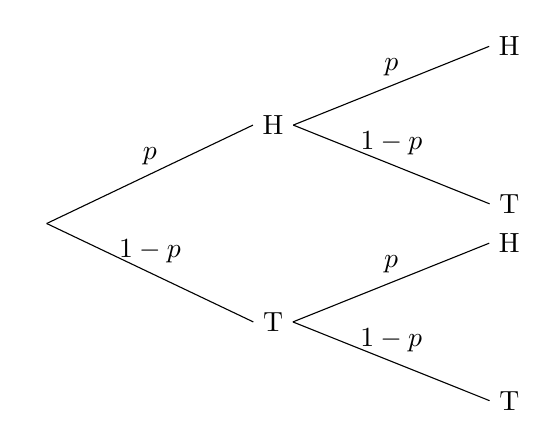
\begin{tikzpicture}[grow'=right,level 1/.style={sibling distance=2.5cm, level distance=3cm},
	level 2/.style={sibling distance=2cm, level distance=3cm}]
	\node {}
	child{
		node {H}
		child{node{H} edge from parent node[above]{$p$}}
		child{node{T} edge from parent node[above,midway]{$1-p$}}
		edge from parent node[above]{$p$}
	}
	child{
		node{T}
		child{node{H} edge from parent node[above]{$p$}}
		child{node{T} edge from parent node[above]{$1-p$}}
		edge from parent node[above]{$1-p$}
	};
	\end{tikzpicture}
\end{center}

All we need to compare is $\Pr(A|B)$ and $\Pr(A)$.
\begin{itemize}
	\item $\Pr(A|B) = p$
	\item $\Pr(A) = p^2 + (1-p)^2$
\end{itemize}

So, the two events are not independent. The reason is quite simple. Suppose that the coin land on heads way more often than tail. If the first coin lands on head, since the second coin lands on head way more often than the tail that means the chance of you getting a match is higher. This means that the information about the first coin tells give you information about the second event.

\theorem (Product Rule)If event $A$ is \emph{independent} of event $B$ then
\[
	\Pr(A \cap B) = \Pr(A) \times \Pr(B)
\]
Some book use this as the definition of independence. The two definiton are equivalent.

\proof There are two cases
\begin{enumerate}[1)]
	\item If $\Pr(B) = 0$ then $\Pr (A \cap B) = 0 = \Pr(A)\Pr(B)$ since $B$ never happen.
	\item If not then we know that
	\[
		\Pr(A\cap B) = \Pr(B)\Pr(A|B) \expl{=}{indep} \Pr(B) \Pr(A)
	\]
\end{enumerate}
\qedd

\theorem Independent is symmetric. If event $A$ is independent of event $B$ then event $B$ is independent of event $A$.

\proof Left for the reader as an exercise
\qedd

\section*{Mutual Independence}

%Let us consider a trial back then before DNA testing. Suppose that the blood of the perpetrator found on the scene has the following properties:(make up number).
%\begin{itemize}
%	\item It is of type O found in 1/10 of the population.
%	\item It is $Rh^-$ found in 1/5 of the population.
%	\item It has of Lewis Le(a+b-) found in 1/4 of the population.
%\end{itemize}
%If the suspect is found to match these three things can we say that the mactching chance is $1/200$? This is not quite the case. We assume independence all the time but it is usually not true. ABO blood type system is found to have a link to Lewis blood type system they are linked to the same gene. That means they are not independent this means you can't multiply all the probability together.

Let us consider consider tossing 3 fair independent coin. Let
\begin{itemize}
	\item $A$ be the event that the 1st and the 2nd coin match.
	\item $B$ be the event that the 2nd and the 3rd coin match.
	\item $C$ be the event that the 1st and the 3rd coin match.
\end{itemize}

Let us see if $A$ and $B$ independent. This is quite easy to see since $\Pr(A) = 1/2$ and $\Pr(B) = 1/2$. $\Pr(A\cap B) = \Pr(HHH) + \Pr(TTT) = 1/4$. So,
\[
	\Pr(A\cap B) = \Pr(A)\Pr(B)
\]
So that means $A$ and $B$ are independent. We can do the same thing for other pairs.
\begin{itemize}
	\item $A$ and $B$ are independent $\Pr(A\cap B) = \Pr(A)\Pr(B)$
	\item $B$ and $C$ are independent $\Pr(B\cap C) = \Pr(B)\Pr(C)$
	\item $A$ and $C$ are independent $\Pr(A\cap C) = \Pr(A)\Pr(C)$
\end{itemize}

The question is can we then conclude that the probability that all three event happens is the product of each probability?
\[
	\Pr(A\cap B \cap C) = \Pr(A) \Pr(B) \Pr(C)
\]
This is not the case since the event that all three event happens is the event that all three coins are the same that means the $\Pr(A\cap B\cap C)=1/4$. But the product of the three is $1/8$. So,
\[
	\Pr(A\cap B \cap C)=\frac{1}{2} \ne \half\times\half\times\half
\]

So, we learn a very important thing that pair wise independent does not imply that the three are \emph{mutually independent}. This leads us to define a stronger assumption.

\definition Event $A_1, A_2, \ldots, A_n$ are \emph{mutually independent} iff $\forall i \forall J \subseteq \{1,2,\ldots, n\}-\{i\}, $
\[
	\Pr(A_i | \bigcap\limits_{j \in J} A_j) = \Pr(A_i).
\]
The symbol looks a bit scary but all it reads is that the probability that any event $A_i$ happens is independent to all possible intersection of all the other events. This definition is a bit hard to work with so let us use another definition.

\definition (Equivalent to above)Event $A_1, A_2, \ldots A_n$ are \emph{mutually independent} iff $\forall J \subseteq \{1,2,\ldots n\}$
\[
	\Pr(\bigcap\limits_{j \in J} A_j) = \prod_{j \in J} \Pr (A_j)
\]
This just say that the probability of any intersection of events is just the product of the probability.

This means that if you need to check for \emph{mutually independent} you need to check all the intersection. Specifically, this means for three events $A_1, A_2, A_3$ we need to check for all of the following
\begin{align*}
	\Pr(A_1 \cap A_2) =& \Pr(A_1) \Pr(A_2)\\
	\Pr(A_1 \cap A_3) =& \Pr(A_1) \Pr(A_3)\\
	\Pr(A_2 \cap A_3) =& \Pr(A_2) \Pr(A_3)\\
	\Pr(A_1 \cap A_2 \cap A_3) =& \Pr(A_1) \Pr(A_2) \Pr(A_3)
\end{align*}
You cannnot skip any of these.

Let us look at another example of tossing tow indpendent dice.
\begin{itemize}
	\item Let $A$ be the event that the first dice is 1,2, or 3.
	\item Let $B$ be the event that the first dice is 3,4, or 5.
	\item Let $C$ be the event that the sum of the two dice is 9.
\end{itemize}

Let us first check the last condition whether
\[
	\Pr(A \cap B \cap C) = \Pr(A) \Pr(B) \Pr(C).
\]
$\Pr(A \cap B \cap C) = \Pr([3,6])=1/36$. $\Pr(A)=1/2$ $\Pr(B)=1/2$ $\Pr(C)=4/36=1/9$. That means
\[
\Pr(A \cap B \cap C) =\frac{1}{36} =\frac{1}{2} \times \frac{1}{2} \times \frac{1}{9}
\]

But, does this means that $A$, $B$ and $C$ are pairwise independent. Unfortunately, no. $\Pr(A\cap B) = 1/6$, $\Pr(A) = 1/2, \Pr(B)=1/2$
\[
	\Pr(A\cap B) \ne \Pr(A) \Pr(B)
\]
So, $A$, $B$ and $C$ are not mutually indpendent.

\end{multicols}


\end{document}
